\documentclass{article}
\usepackage{graphicx}
\usepackage{hyperref}
\usepackage{xcolor}

\graphicspath{ {images/} }
\begin{document}
\pagecolor{white}

\title{%
  Study, understand and use GCM \\
  \large HW3 - CNS Sapienza}

\author{Giulio Serra 1904089}
\date{November 21, 2019}

\maketitle

\begin{titlepage}
\end{titlepage}

\tableofcontents

\begin{titlepage}
\end{titlepage}

\section{Introduction}\label{sec:intro}
The aim of this essay is to describe the features and functionality of Galois/Counter Mode(GCM) comparing the performances with the CBC mode while using a 256 bit AES Cipher .\\

\section{Galois/Counter Mode}\label{sec:gcm}

GCM is a modern 128b block cipher mode of operation with notable good performances, that can be achieved even with minimum hardware resources, this made GCM particularly good for mobile use as it's low hardware costly and his high speed throughput  makes it good for the use on communication channels.\\\\
GCM's messages can be authenticated using GMAC(Galois authentication codes) that operates with incremental messaging authentication codes, all the features described above means that GCM can assure both confidentiality and authenticity.
A big part of GCM security comes over the initialization vector (IV) thats need to be different with every encryption, this assure that the encrypted block is almost the same as a random permutation of the plain text (so patterns are really difficult to spot).

	\begin{figure}[h]
		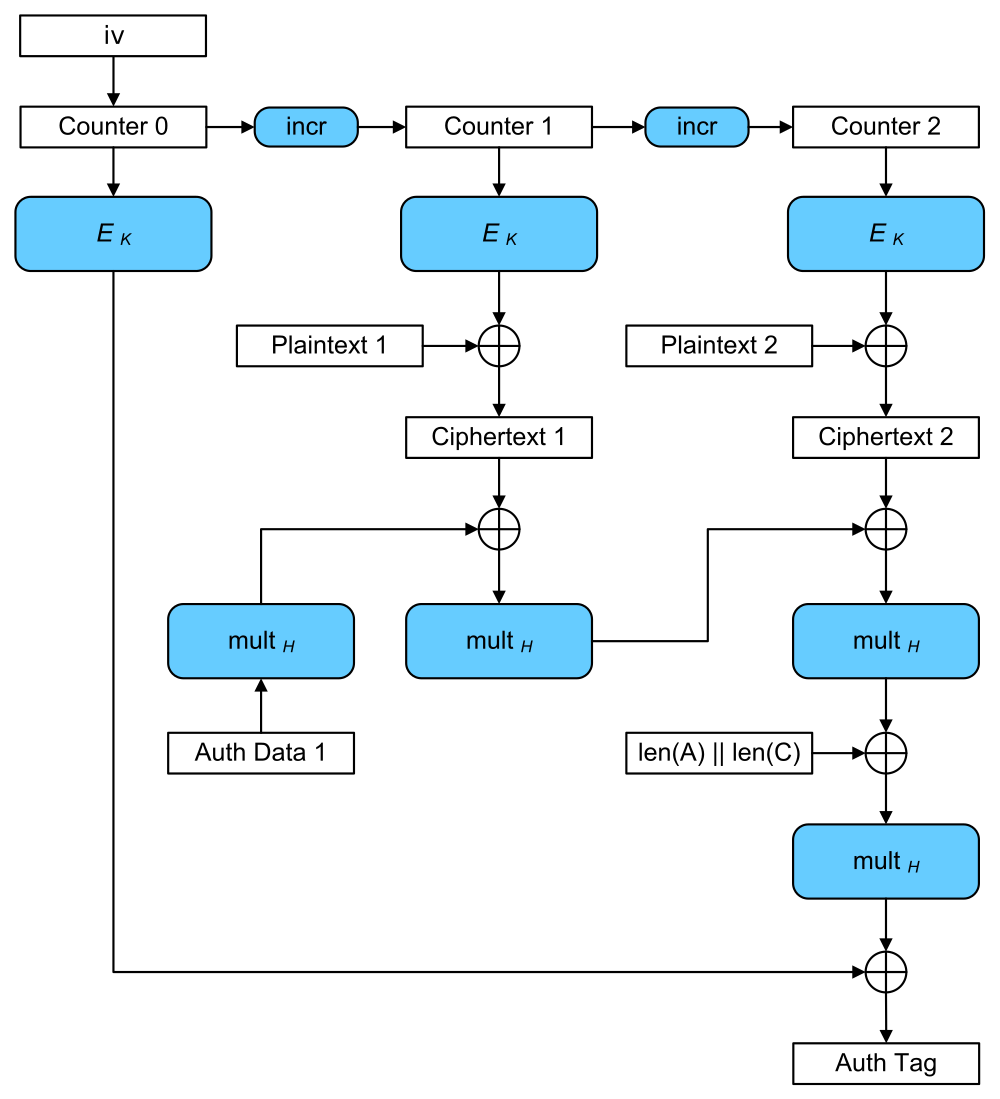
\includegraphics[width=0.6\textwidth ]{images/GCM.png}
		\centering
		\caption{Basic operations of GCM}
	\end{figure}

\clearpage
\subsection{Mathematical Functions of GCM}\label{sec:mathgcm}

GCM relies on counter modes and Galois modes of authentication.\\
In counter modes a stream cipher is generated starting from a block cipher by encrypting sequentially chunks of a counter vector(a function that produce a vector with element that does not repeat for a long time), then the encrypted block is XORED with the plain text outputting a cipher text; note that counter modes ticks all the wright boxes because is : parallelizable both in encryption and decryption and can be random accessed.
The authentication tag is constructed by using the GHASH function that takes as input the hash key (H), consisting in a 128b encrypted block cipher, the data(A) and the cipher text (C):


\begin{center}
\[{{GHASH}}(H,A,C)=X_{m+n+1}\] 
\end{center}
 
 This type of authentication rely on the Galois Field multiplication that is an operation done in a set of finite elements where all the elements are well known: in particular here is the polinomial used to define 
\[{GF(2^{128} ) }\] 

\begin{center}
 is:  
 \end{center}
 
 \[{x^{128}+x^{7}+x^{2}+x+1 }\] 
 
 this is operation is so fast because the multiplication can be parallelized.
 
\section{CBC Operating Mode}\label{sec:cbcop}
The cipher block chaining mode (already discussed in HW1) is an operating mode where each block of plaintext is XORED with the previous cipher text block: while the first block still uses an Initialization vector to compute the first encrypted block. The same operation is done in decryption(starting from the cyphertext).\\
The main issue with CBC is that while the decryption can in fact, be parallelized(because the cipher text is already been computed), in encryption we need to wait for each block to be encrypted, to compute the next one: this can result in significant slow downs in performances.
As for error recovery:  if in decryption an incorrect IV is used this can result in incorrect first block, but if the key is correct, the following blocks output as normal, the same things happen in a bit in cipher text block is changed: the following blocks output as normal.


	\begin{figure}[h]
		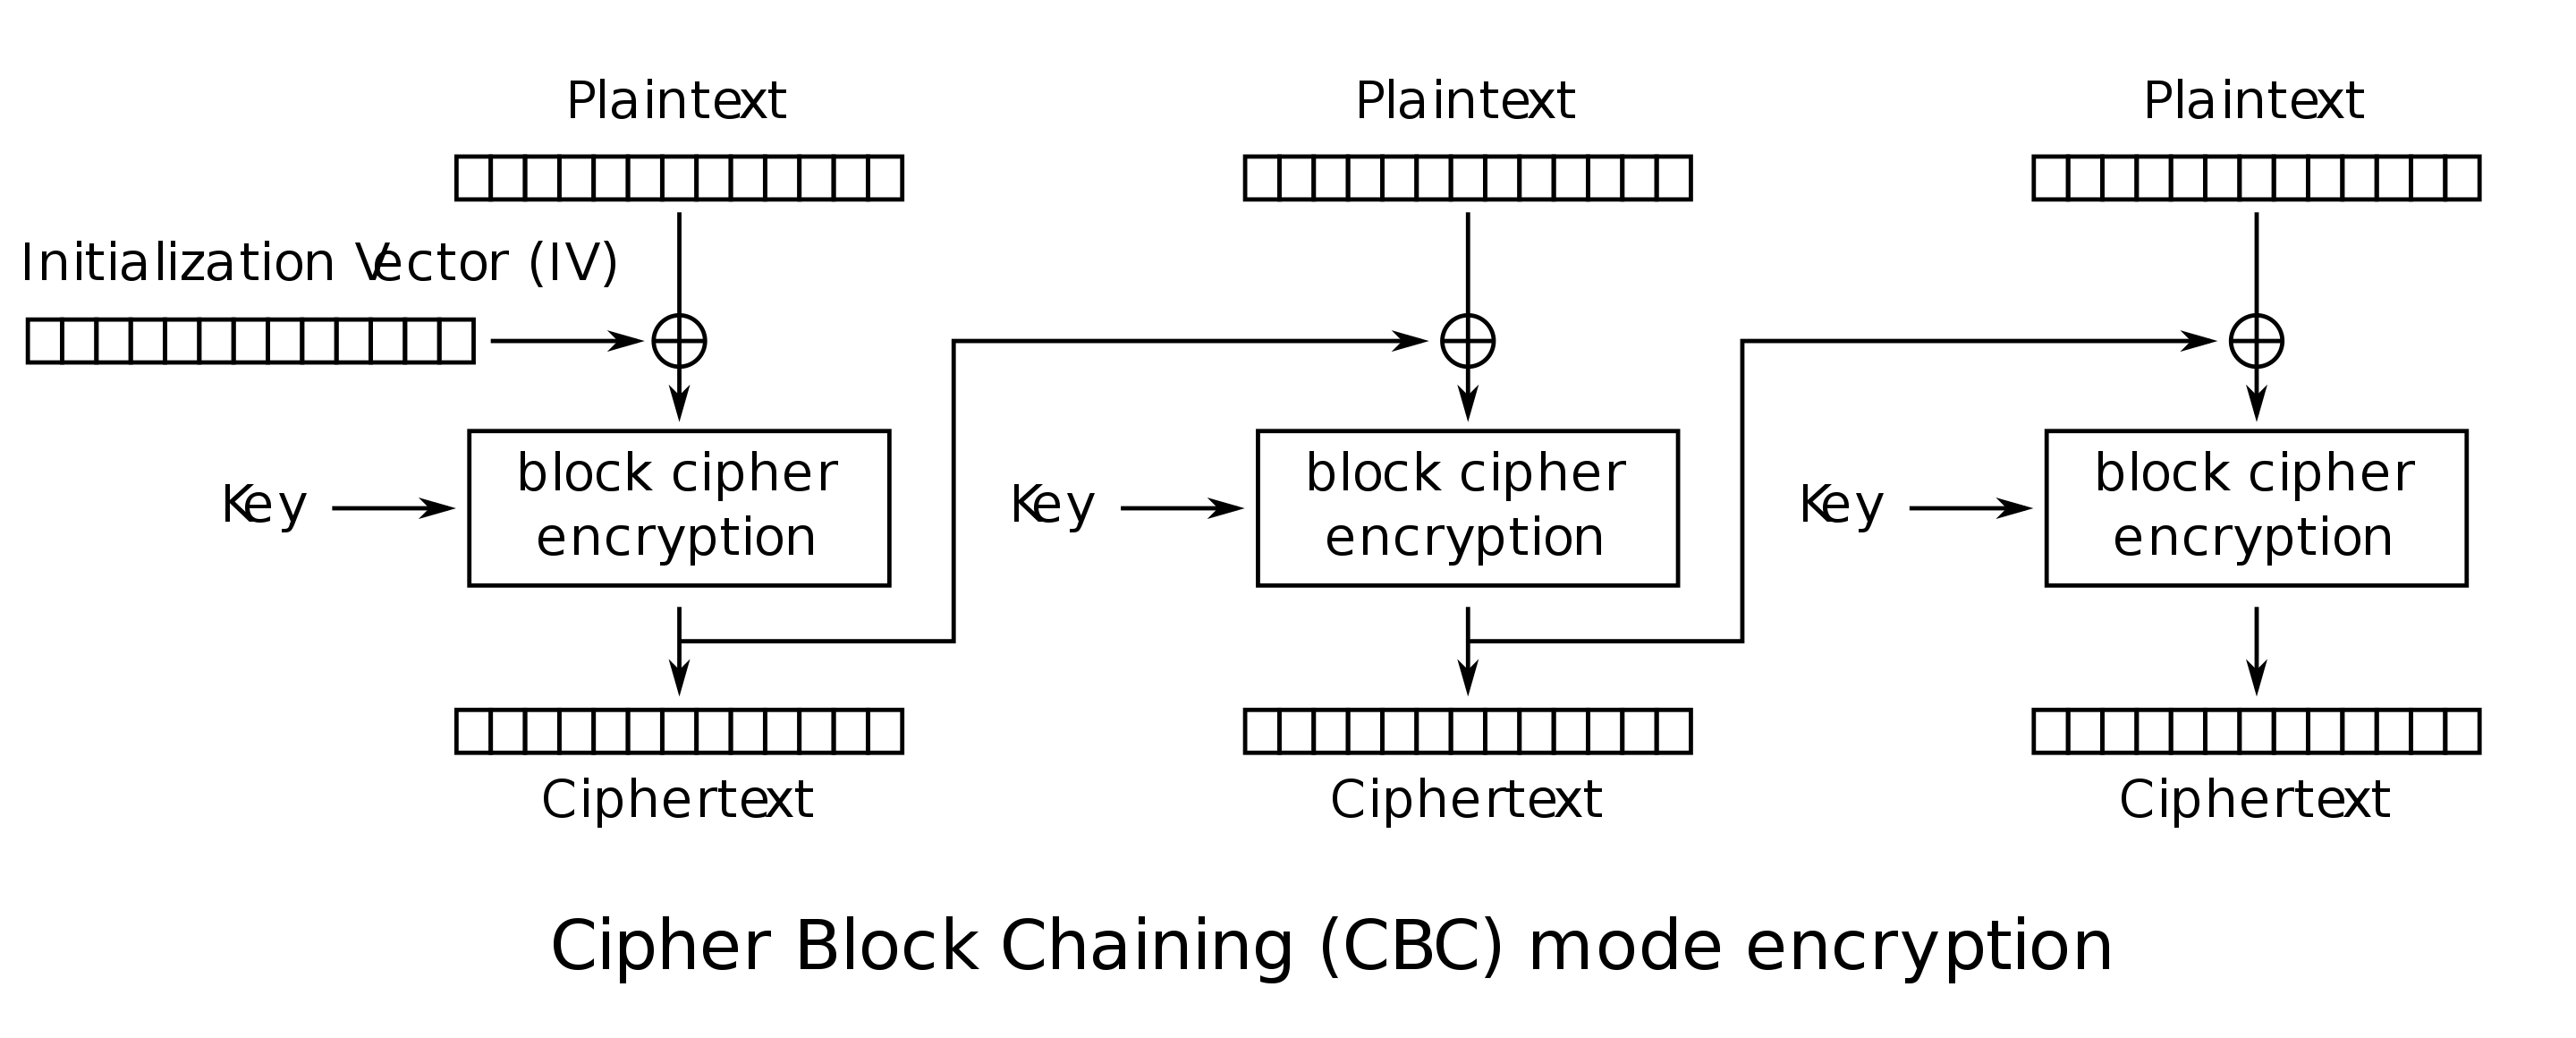
\includegraphics[width=1\textwidth ]{images/CBC_enc.png}
		\centering
	\end{figure}
	
	
	\begin{figure}[h]
		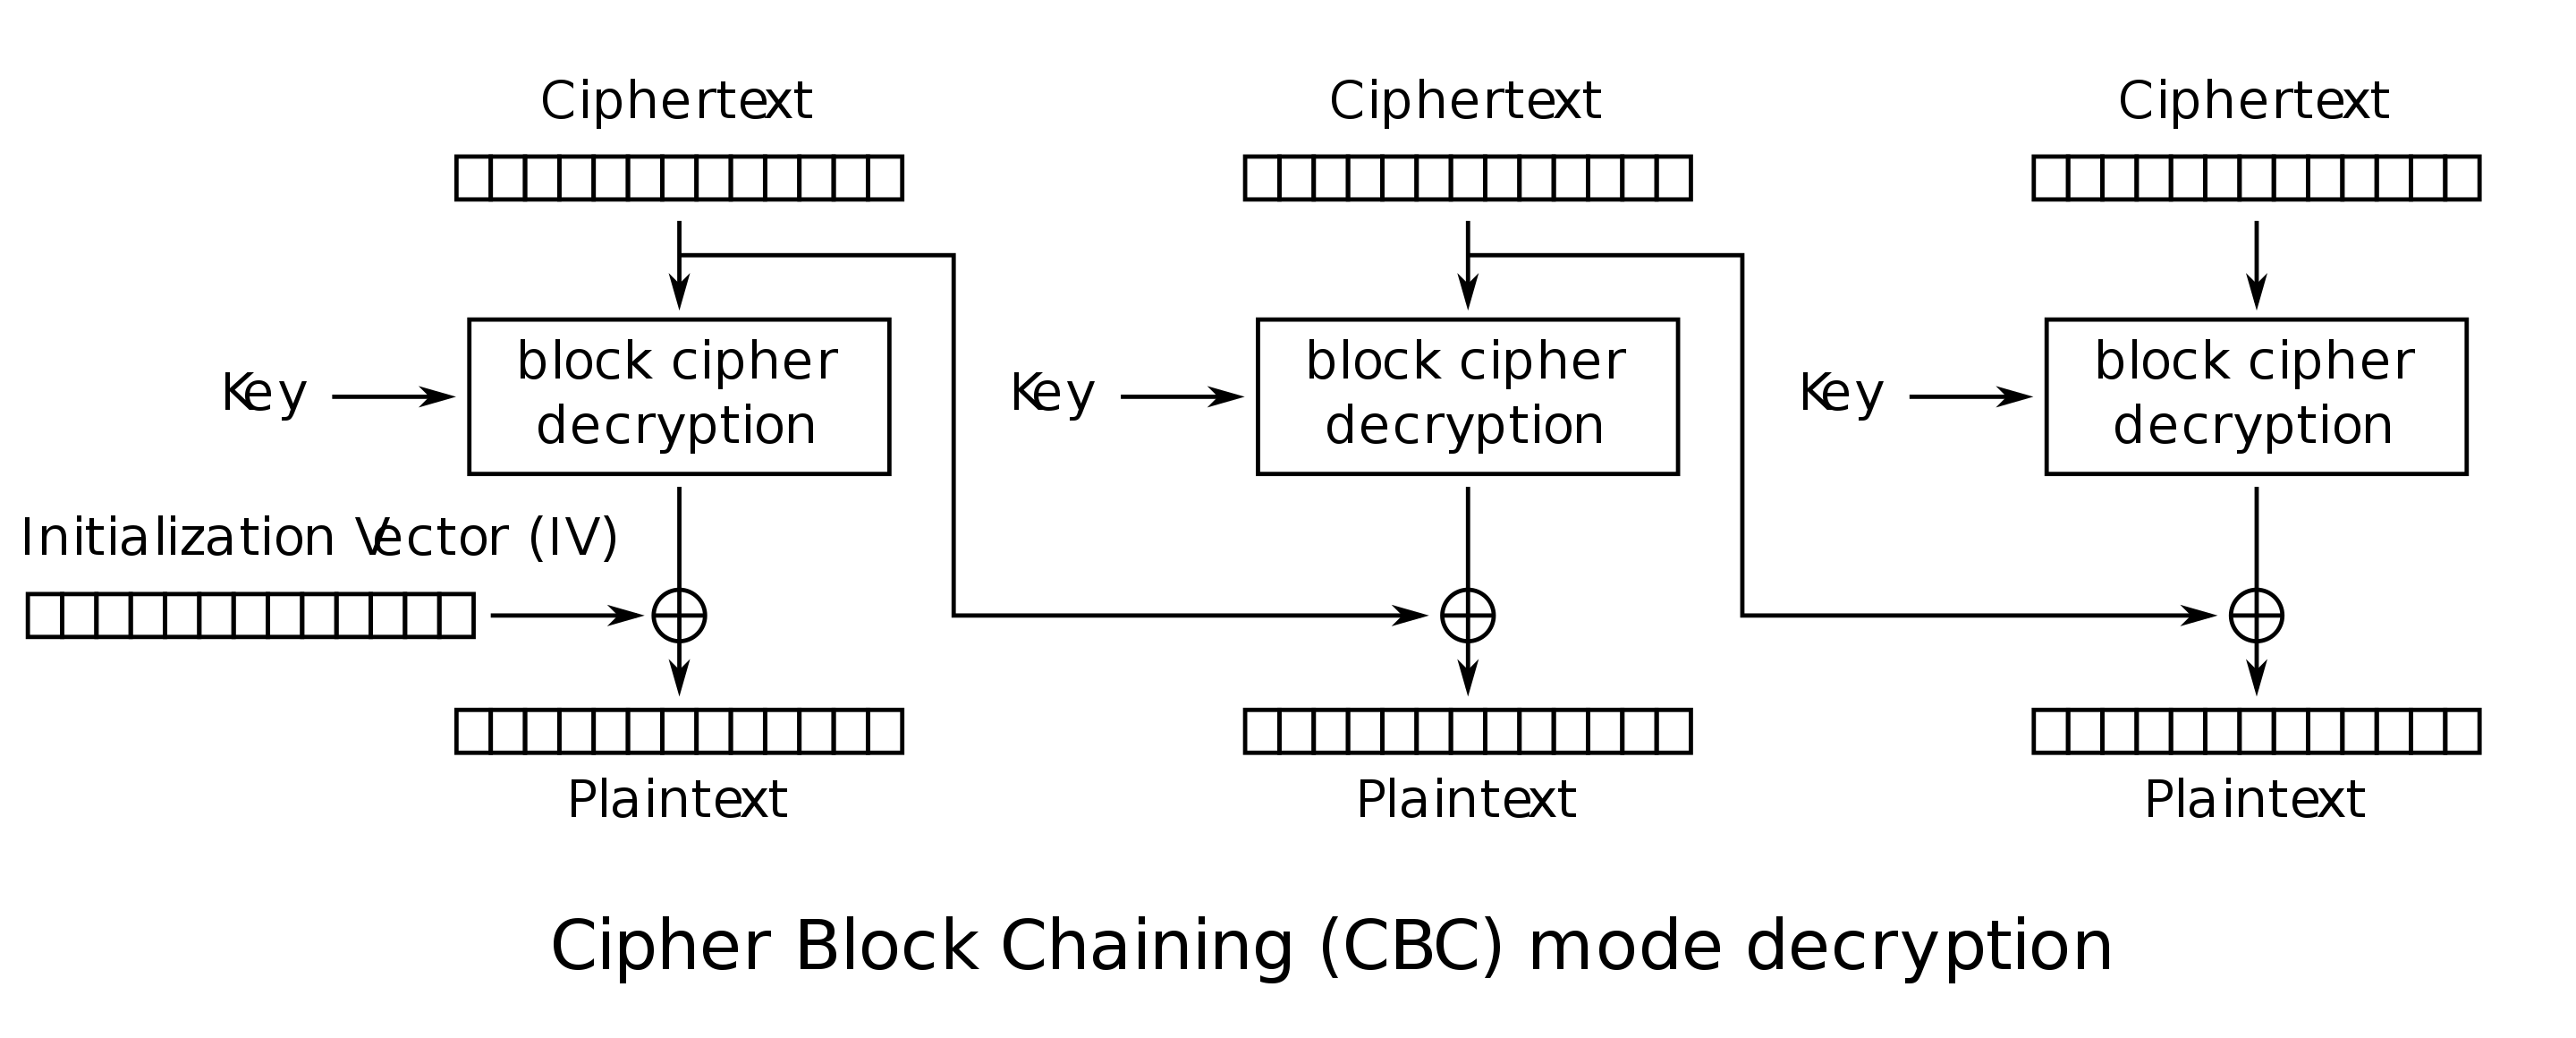
\includegraphics[width=1\textwidth ]{images/CBC_dec.png}
		\centering
	\end{figure}


\clearpage

\subsection{Mathematical Functions of CBC}

The basic of the CBC operating mode is the XOR operation, both in encryption and decryption the first block is taken directly from the Initialization Vector : \[C_{0} = IV\]  while in decryption the i-plaintext block is
\[{\ P_{i}=D_{K}(C_{i})\oplus C_{i-1},}\] where: \[P_{i}\] is the plaintext resulted from the XOR operation between the decryption of the current cipher text block and the previous cipher text block(Ci-1). 
During the encryption: \[{\ C_{i}=E_{K}(P_{i}\oplus C_{i-1}),}\] the current cipher text block of the iteration, is the result of the XOR operation between the current plaint text block and the previous encrypted block.

\section{Performances Evaluation}

In order to evaluate how the parallelization of the encryption affect the performances of GCM against the more common CBC, we can write a simple script to perform an encryption and a decryption of a 100mb  text file, unfortunately the widely popular OpenSSL library still does not support the GCM mode of operation, we need to use the OpenLibreSSL library to access the beta version of this mode of operation.

\subsection{Implementation}
Here follow a simple implementation of two consecutive encryption/decryption using 256b AES Cipher on a 100Mb text file:

\begin{verbatim}
#!/bin/bash
PATH="/usr/local/opt/libressl/bin:$PATH"
INPUT='/Users/giulioserra/Documents/Universita/CNS3/plaintext.txt'
OUTPUT_CBC='/Users/giulioserra/Documents/Universita/CNS3/cipherCBC.enc'
OUTPUT_GCM='/Users/giulioserra/Documents/Universita/CNS3/cipherGCM.enc'
OUTPUTPLAIN='/Users/giulioserra/Documents/Universita/CNS3/decCBC.txt'
OUTPUTPLAIN_GCM='/Users/giulioserra/Documents/Universita/CNS3/decGCM.txt'
KEY='learning'

echo "Starting AES 256 CBC..."
start_CBC=$SECONDS

ENCRYPTION_CBC=$(openssl enc -aes-256-cbc -pbkdf2 -e -in $INPUT 
-out $OUTPUT_CBC -k $KEY)

duration_ECBC=$(( $SECONDS - start_CBC))
dt_min=$(printf %.3f $(echo "$duration_ECBC" | bc -l))

echo "file encrypted with AES CBC, elapsed time: $dt_min s"; 

start_CBC_DEC=$SECONDS
DECRIPTION=$(openssl enc -aes-256-cbc -pbkdf2 -d -in $OUTPUT_CBC 
-out $OUTPUTPLAIN -k $KEY)

duration_DCBC=$(( $SECONDS - start_CBC_DEC))
dt_min_dec=$(printf %.3f $(echo "$duration_DCBC" | bc -l))

echo "file decrypted with AES CBC, elapsed time: $dt_min_dec s"; 

echo "---------------------------------------------------------------------------------"; 

echo "Starting AES 256 GCM..."
start_GCM=$SECONDS
ENCRYPTION_GCM=$(libressl enc -aes-256-gcm -pbkdf2 -e 
-in $INPUT -out $OUTPUT_GCM -k $KEY)



duration_EGCM=$(( $SECONDS - start_GCM))
dt_GCM_enc=$(printf %.3f $(echo "$duration_EGCM" | bc -l))

echo "file encrypted with AES GCM, elapsed time: $dt_GCM_enc s"; 

start_CBC_GCM=$SECONDS
DECRIPTION=$(libressl enc -aes-256-gcm -pbkdf2 -d -in $OUTPUT_GCM 
-out $OUTPUTPLAIN_GCM -k $KEY)

duration_DGCM=$(( $SECONDS - start_CBC_GCM))
dt_min_gcm_dec=$(printf %.3f $(echo "$duration_DGCM" | bc -l))

echo "file decrypted with AES GCM, elapsed time: $dt_min_gcm_dec s"; 

Starting AES 256 CBC...
file encrypted with AES CBC, elapsed time: 0,000 s
file decrypted with AES CBC, elapsed time: 1,000 s
---------------------------------------------------------------------------------
Starting AES 256 GCM...
file encrypted with AES GCM, elapsed time: 0,000 s
file decrypted with AES GCM, elapsed time: 0,000 s
\end{verbatim}

The result of the execution clock the encryption using CBC at around 1.0 seconds, while doing instantaneously the decryption.
In GCM mode both encryption and decryption are instantaneous.\\
This results may contradict what stated in paragraph 1 and 2 (in CBC mode the decryption should be faster than the encryption), this may have something to do on how the library use the parallelization so the result can vary between OS and different architectures.\\To fully appreciate the differences between the two operating mode, we can use a variation of the same script on a 1GB file:

\begin{verbatim}
Starting AES 256 CBC...
file encrypted with AES CBC, elapsed time: 4,000 s
file decrypted with AES CBC, elapsed time: 3,000 s
---------------------------------------------------------------------------------
Starting AES 256 GCM...
file encrypted with AES GCM, elapsed time: 2,000 s
file decrypted with AES GCM, elapsed time: 3,000 s


\end{verbatim}
Finally we get some expected results: in fact the decryption is faster than the encryption (because of the parallelization) in CBC mode, while being slower that GCM mode using the same AES 256 Cipher.

\section{References}

	Galois Counter Mode:\\
	 \verb|https://en.wikipedia.org/wiki/Galois/Counter_Mode|\\
	 \\CBC Mode:\\
	 \verb|https://en.wikipedia.org/wiki/Block_cipher_mode_of_operation|\\
	\\The LibreSSL Library:\\
	 \verb|https://www.libressl.org|\\
	 \\1GB Test file:\\
	 \verb|https://speed.hetzner.de|\\
	

\end{document}